\documentclass{article}

\usepackage[brazil]{babel}

\usepackage{amsmath, amssymb}
\usepackage{graphicx}
\usepackage[colorlinks=true, allcolors=blue]{hyperref}

\usepackage{listings}
\lstset{
basicstyle=\small\ttfamily,
columns=flexible,
breaklines=true
}

\usepackage[section]{placeins}

\usepackage{tcolorbox}

\title{Relatório 03}
\author{Vinícius de Oliveira Peixoto Rodrigues (245294)}
\date{Março de 2023}

\begin{document}
\maketitle

\section{Introdução}

No modelo OSI, que segmenta em diferentes camadas os componentes
e processos de um sistema de comunicação, define-se como a \textbf{camada 4}, ou \textbf{camada de transporte}, o conjunto de protocolos e serviços cujo
objetivo é prover um canal de comunicação host-a-host para uso de
aplicações. Nessa camada, os protocolos fornecem serviços como confiabilidade,
controle de fluxo, multiplexão e \textit{streams} de dados orientadas a
conexão.

Nessa camada, os dois protocolos mais importantes são o TCP
(\textit{Transmission Control Protocol}) e UDP \textit{User Datagram Protocol}.
O TCP busca oferecer uma stream de bytes confiável, orientada a conexão,
ordenada e com checagem de erros; além disso,
o protocolo implementa também funcionalidades para controle de
congestionamento de rede. O UDP, por outro lado, é significativamente
mais simples, fornecendo funcionalidades de transporte de mensagens
(datagramas) sem o conceito de conexão, ordenamento ou controle de fluxo.
O UDP, assim como o TCP, fornece checagem de integridade por meio
de checksums.

\section{Objetivos}

O objetivo geral deste experimento é explorar o funcionamento dos
protocolos TCP e UDP. Em particular, os objetivos específicos do
experimento são:

\begin{itemize}
    \item Analisar o conteúdo de pacotes TCP e UDP por meio
          da ferramenta Wireshark
    \item Estudar o processo de three-way handshake do protocolo
          TCP, assim trocas de pacotes envolvidas no processo
    \item Investigar os mecanismos de controle de fluxo do TCP por
          meio da geração de tráfego usando a ferramenta ITGSend
\end{itemize}

\begin{itemize}
    \item Explorar as funcionalidades da ferramenta \texttt{mininet-wifi}
    \item Compreender os princípios básicos de funcionamento de arquiteturas
          de rede wireless
    \item Fazer uso do simulador para investigar a relação entre parâmetros
          físicos e a performance de redes sem fio
\end{itemize}

\section{Metodologia}

O experimento dividiu-se em sete etapas:

\subsection{Primeiros passos}

Foi realizada a criação de uma topologia wireless básica, com um AP e duas estações
(\texttt{sta1} e \texttt{sta2}).
Em seguida, foram realizados testes básicos de conexão e desconexão entre as estações
e o access point; finalmente, foram realizadas medições de largura de banda entre as
duas estações.

\subsection{Exploração dos parâmetros do simulador}
Foi explorado o ajuste de parâmetros das estações no simulador, em particular o de
posição das estações. Além disso, foi realizada uma análise dos diversos parâmetros
de configuração disponíveis no simulador.


\subsection{Visualização da topologia wireless}




\subsection{Análise de quadros}
Análise de quadros 802.11 gerados pelo simulador no Wireshark


\section{Resultados e Discussão}

\subsection*{Parte 1}

\begin{tcolorbox}
    Qual é o atraso observado entre \texttt{sta1} e \texttt{sta2}?
    Houve perda de pacotes no canal? Justifique suas respostas de forma objetiva.
\end{tcolorbox}

\begin{figure}[!htb]
\centering
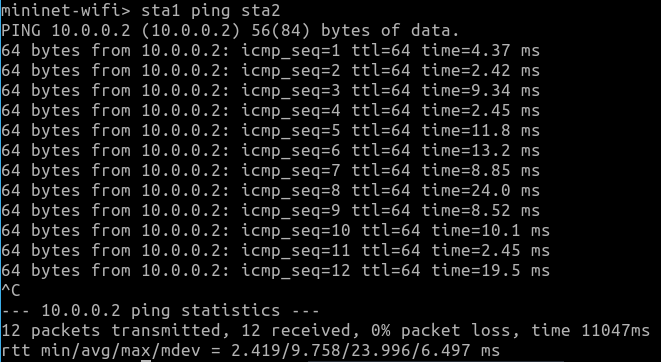
\includegraphics[width=\columnwidth]{images/p1_ping.png}
\caption{\texttt{ping} entre \texttt{sta1} e \texttt{sta2}.}
\end{figure}

O atraso médio observado na saída do comando \texttt{ping} é de 9.8 segundos.
Além disso, não foram observadas perdas de pacote.

\begin{tcolorbox}
    Use a ferramenta iperf para avaliar a banda disponível (Mbps)
    entre sta1 e sta2.
\end{tcolorbox}

\begin{figure}[!htb]
\centering
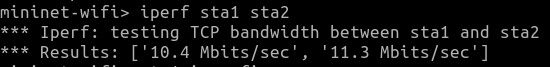
\includegraphics[width=\columnwidth]{images/p1_iperf.png}
\caption{Teste de largura de banda entre \texttt{sta1} e \texttt{sta2}.}
\end{figure}

\end{document}
